\documentclass{beamer}
\mode<presentation> {

% The Beamer class comes with a number of default slide themes
% which change the colors and layouts of slides. Below this is a list
% of all the themes, uncomment each in turn to see what they look like.

%\usetheme{default}
%\usetheme{AnnArbor}
%\usetheme{Antibes}
%\usetheme{Bergen}
%\usetheme{Berkeley}
%\usetheme{Berlin}
%\usetheme{Boadilla}
%\usetheme{CambridgeUS}
%\usetheme{Copenhagen}
%\usetheme{Darmstadt}
\usetheme{Dresden}  %FIRST PREFERENCE
%\usetheme{Frankfurt}
%\usetheme{Goettingen}
%\usetheme{Hannover}
%\usetheme{Ilmenau}
%\usetheme{JuanLesPins}
%\usetheme{Luebeck}
%\usetheme{Madrid}
%\usetheme{Malmoe}
%\usetheme{Marburg}
%\usetheme{Montpellier}
%\usetheme{PaloAlto}
%\usetheme{Pittsburgh}
%\usetheme{Rochester}
%\usetheme{Singapore}
%\usetheme{Szeged}
%\usetheme{Warsaw}

% As well as themes, the Beamer class has a number of color themes
% for any slide theme. Uncomment each of these in turn to see how it
% changes the colors of your current slide theme.

%\usecolortheme{albatross}
%\usecolortheme{beaver}
%\usecolortheme{beetle}
%\usecolortheme{crane}
%\usecolortheme{dolphin}
%\usecolortheme{dove}
%\usecolortheme{fly}
%\usecolortheme{lily}
%\usecolortheme{orchid}
%\usecolortheme{rose}
%\usecolortheme{seagull}
%\usecolortheme{seahorse}
\usecolortheme{whale} %FIRST PREFERENCE
%\usecolortheme{wolverine}

%\setbeamertemplate{footline} % To remove the footer line in all slides uncomment this line
%\setbeamertemplate{footline}[page number] % To replace the footer line in all slides with a simple slide count uncomment this line

%\setbeamertemplate{navigation symbols}{} % To remove the navigation symbols from the bottom of all slides uncomment this line
}
%\usetikzlibrary
\def\nbrcircles {377}
\def\outerradius {30mm}
\def\deviation {.9}
\def\fudge {.62}

\newcounter{cumulArea}
\setcounter{cumulArea}{0}

%\usepackage[dvipsnames]{xcolor}
%\usepackage{pgfplots}
%\pgfplotsset{width=8cm,compat=newest}
\usepackage{smartdiagram}
\usepackage{tcolorbox}
\usetikzlibrary{arrows}
\usepackage[european]{circuitikz}
\usepackage{siunitx}
\hypersetup{pdfpagemode=FullScreen}
\usepackage{graphicx} % Allows including images
\usepackage{booktabs} % Allows the use of \toprule, \midrule and \bottomrule in tables
%\usepackage[pdftex,
            %pdftitle={Hitesh's PPT},
            %pdfsubject={Personal %Workbook},
            %pdfproducer={Not a Robot},
            %pdfcreator={Hitesh's System}]{hyperref}
%----------------------------------------------------------------------------------------
%	TITLE PAGE
%----------------------------------------------------------------------------------------
\title[Project Presentation]{Analysis of Sustained Phonation of Person with Voice Disorder} % The short title appears at the bottom of every slide, the full title is only on the title page
\author{Hitesh A H} % Your name
\institute[Government Engineering College, Barton Hill] % Your institution as it will appear on the bottom of every slide, may be shorthand to save space
{
\textit{TRV20ECSPXX, Signal Processing} \\\textit{Department of Electronics and Communication Engineering} \\ % Your institution for the title page
\medskip
%\textit{bofu20131@163.com} % Your email address
}
\date{\today} % Date, can be changed to a custom date

\begin{document}

\begin{frame}
\titlepage % Print the title page as the first slide
\end{frame}

\begin{frame}
\frametitle{Overview} % Table of contents slide, comment this block out to remove it
\tableofcontents % Throughout your presentation, if you choose to use \section{} and \subsection{} commands, these will automatically be printed on this slide as an overview of your presentation
\end{frame}

%----------------------------------------------------------------------------------------
%	PRESENTATION SLIDES
%----------------------------------------------------------------------------------------

%------------------------------------------------
\section{Research Problem} 
\begin{frame}
\frametitle{Introduction}
\begin{itemize}
    \item The \textbf{human voice} is a wonderfully, perhaps uniquely, expressive instrument, exhibiting a bewildering number of expressive variations beyond those of pitch and loudness, including trill, effort level etc.
    \item The speech represents an intrinsic characteristic of human behaviour. Any disturbances in the normal speech of a human being are called \textbf{speech disorder}.
    \item Automatic detection and assessment of voice disorders is important in diagnosis and treatment planning of voice disorders.
\end{itemize}
\end{frame}
\begin{frame}{Introduction}
    \begin{enumerate}
    \setbeamertemplate{enumerate items}[square]
    %\setbeamercolor{item projected}{bg=magenta!70!black,fg=white}
    %\setbeamercolor{enumerate subitem}{fg=red!80!black}
        \item Speech production requires airflow from the lungs to be phonated through vocal folds of the larynx and resonated in the vocal cavities shaped by the tongue, jaw, soft palate, lips, and other articulators. 
        \item Phonation is a process by which the vocal folds produce certain sounds through quasi-periodic vibration(voicing).
        \item Any abnormality in the larynx that affect voicing in speech production: \textbf{Voice disorder}.
    \end{enumerate}
\end{frame}
\begin{frame}{Significance}
\begin{itemize}
    \item According to American speech-language-hearing association, voice disorders: \textbf{organic} \& \textbf{neurological}.
    \item Affects communication and social integration: patients will also have psychological and emotional issues. Deterioration of the quality of life.
    \item Expensive tests like video or laryngoscopy/ stroboscopy.
    \item Hence, early detection of speech disorder is of utmost importance.
\end{itemize}
\end{frame}
\begin{frame}{From Literature}
\textbf{Article:}\textit{Prevalence of Voice Disorders in School Teachers in a District in South India}
\begin{tcolorbox}[colback=green!5,colframe=green!40!black,title=Results]
Teachers reporting a current voice complaint at the time of study were administered the validated vernacular version of the voice handicap index questionnaire (VHI 30). 702 teachers, The reported prevalence was 45.4\% for present difficulty related to their voice, 52.8\% for some voice problem in the last 1 year[2019], and 70.1\% for problems experienced during the duration of their teaching career.
\end{tcolorbox}
\end{frame}
\begin{frame}{Field Overview}
\centering
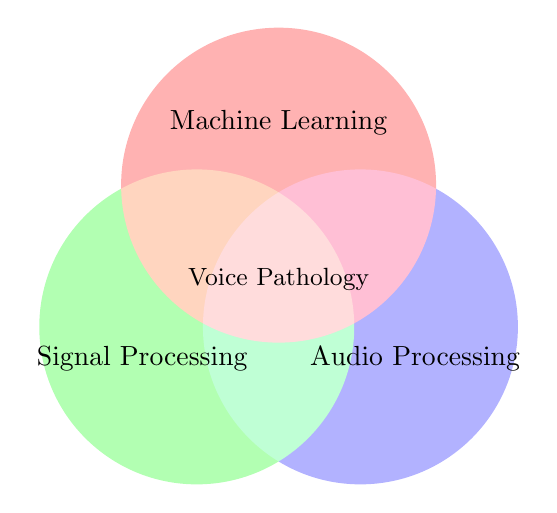
\begin{tikzpicture}
  \begin{scope}[blend group = soft light]
    \fill[red!30!white]   ( 90:1.2) circle (2);
    \fill[green!30!white] (210:1.2) circle (2);
    \fill[blue!30!white]  (330:1.2) circle (2);
  \end{scope}
  \node at ( 90:2)    {Machine Learning};
  \node at ( 210:2)   {Signal Processing};
  \node at ( 330:2)   {Audio Processing};
  \node [font=\small] {Voice Pathology};
\end{tikzpicture}
    
\end{frame}
\section{Literature Review}
\begin{frame}{Citation Graph}
    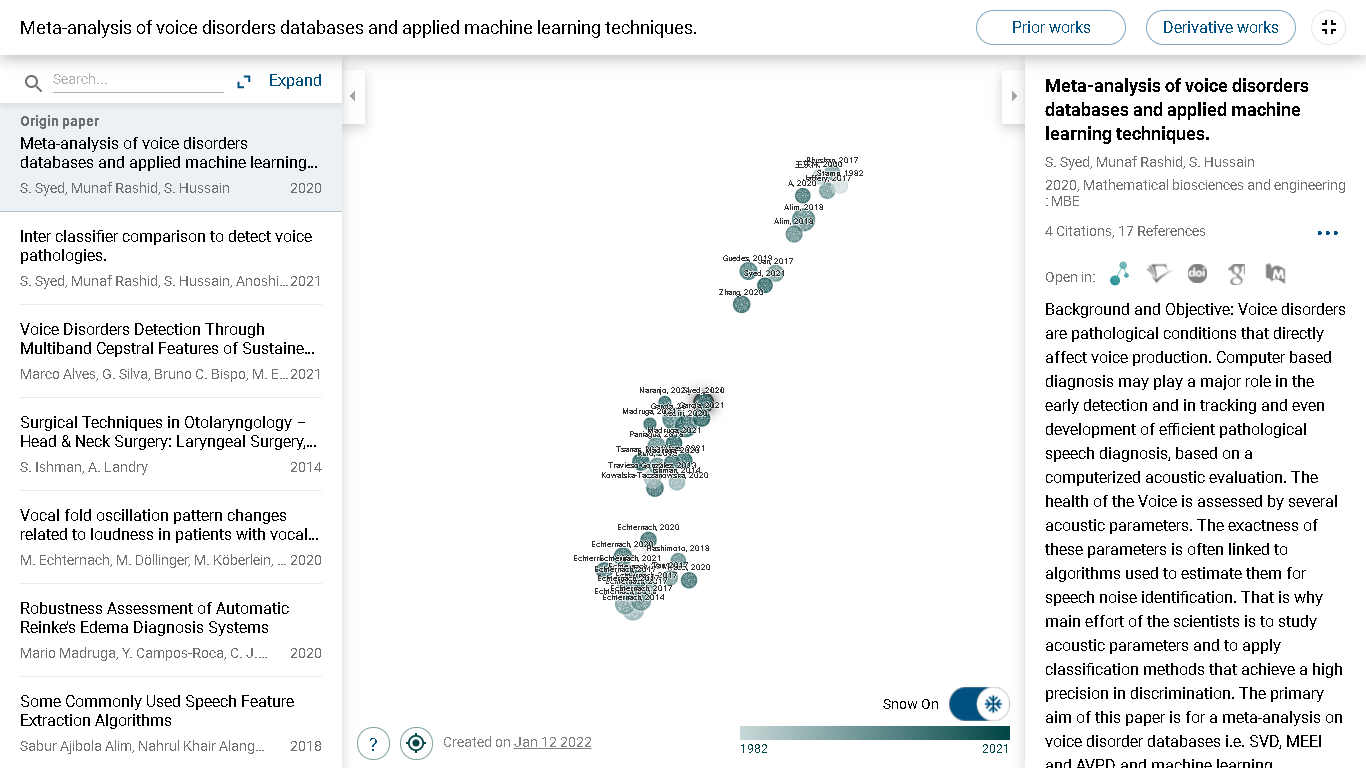
\includegraphics[width=\textwidth]{pic1}
\end{frame}
\begin{frame}{Research so far..}
\centering
    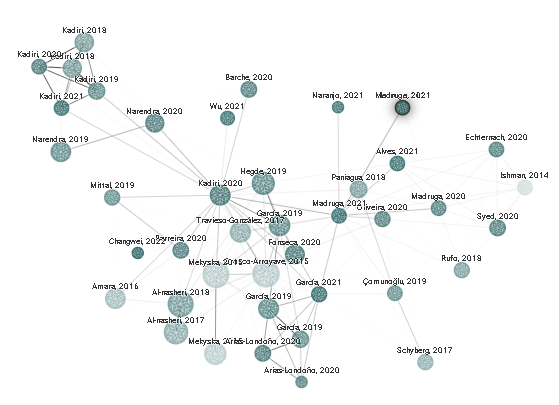
\includegraphics[width=9cm, height=6cm]{cite2.PNG}
    \\\tiny Source: \textit{\href{https://www.connectedpapers.com/}{Connected Papers}}
\end{frame}
\begin{frame}{Comparison Summary}
\small \textbf{Article:} \textit{] Pavol Harar, Jesus B. Alonso-Hernandez, Jiri Mekyska, Zoltan Galaz, Radim Burget and Zdenek Smekal: Voice Pathology Detection Using Deep Learning: a Preliminary Study}
\\\small\textbf{Ext. features:} RMS energy \& PCM loudness
\\\small\textbf{Classifier:} SVM
\\\small\textbf{Accuracy:} \textcolor{red}{71.3\%}
\end{frame}
\begin{frame}{Comparison Summary}
\small \textbf{Article:} \textit{] Alireza Bayestehtashk, Meysam Asgaria, Izhak Shafran, James McName: Fully automated assessment of the severity of Parkinson’s disease from speech}
\\\small\textbf{Ext. features:} pitch frequency, jitter, shimmer \& MFCC
\\\small\textbf{Classifier:} Open SMILE
\\\small\textbf{Accuracy:} \textcolor{red}{91.8\%}
\end{frame}
\begin{frame}{Comparison Summary}
\small \textbf{Article:} \textit{J. R. Orozco-Arroyave, Florian Hönig, J. D. Arias-Londoño, J. F. Vargas-Bonilla1 and Elmar Nöth : Spectral and cepstral analyses for Parkinson’sdisease detection in Spanish vowels and words. Expert Systems}
\\\small\textbf{Ext. features:} LPC, MFCC
\\\small\textbf{Classifier:} SVM with Gaussian Kernal 
\\\small\textbf{Accuracy:} \textcolor{red}{80-92\%}
\end{frame}
\begin{frame}{Key Points}
\begin{itemize}
    \item  In literature, widely used system features are: Mel Frequency Cepstral Co-efficient (\textcolor{red}{MFCC}), perceptual linear prediction (PLP), and Linear Prediction Cepstral Coefficient (\textcolor{red}{LPCC}) ~ reliable acoustic measures of voice impairment.
    \item Adversarial Instance have Robust Model with \textcolor{red}{minimum error}.
    \item Closed domain adaptation with fine tuning. 
\end{itemize}
\end{frame}
\begin{frame}{Feature extraction approaches in voice disorder detection}
\centering
\tikzset{every picture/.style={line width=0.75pt}} %set default line width to 0.75pt        

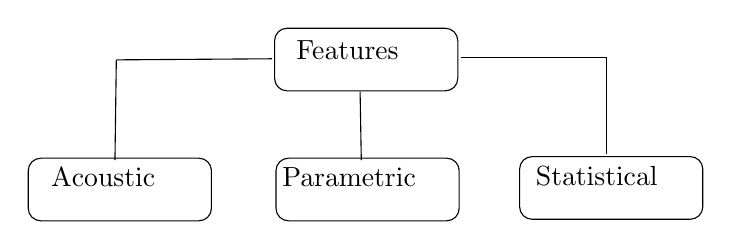
\begin{tikzpicture}[x=0.75pt,y=0.75pt,yscale=-1,xscale=1]
%uncomment if require: \path (0,300); %set diagram left start at 0, and has height of 300

%Rounded Rect [id:dp3541801385827523] 
\draw   (354.7,62.24) .. controls (354.7,58.91) and (357.4,56.21) .. (360.73,56.21) -- (436.93,56.21) .. controls (440.26,56.21) and (442.97,58.91) .. (442.97,62.24) -- (442.97,80.35) .. controls (442.97,83.68) and (440.26,86.38) .. (436.93,86.38) -- (360.73,86.38) .. controls (357.4,86.38) and (354.7,83.68) .. (354.7,80.35) -- cycle ;
%Rounded Rect [id:dp6609580820178511] 
\draw   (355.36,124.86) .. controls (355.36,121.53) and (358.06,118.82) .. (361.4,118.82) -- (437.59,118.82) .. controls (440.93,118.82) and (443.63,121.53) .. (443.63,124.86) -- (443.63,142.96) .. controls (443.63,146.3) and (440.93,149) .. (437.59,149) -- (361.4,149) .. controls (358.06,149) and (355.36,146.3) .. (355.36,142.96) -- cycle ;
%Rounded Rect [id:dp7777021712740482] 
\draw   (472.73,124.1) .. controls (472.73,120.77) and (475.43,118.07) .. (478.77,118.07) -- (554.96,118.07) .. controls (558.3,118.07) and (561,120.77) .. (561,124.1) -- (561,142.21) .. controls (561,145.54) and (558.3,148.25) .. (554.96,148.25) -- (478.77,148.25) .. controls (475.43,148.25) and (472.73,145.54) .. (472.73,142.21) -- cycle ;
%Rounded Rect [id:dp04153998952330462] 
\draw   (236,124.86) .. controls (236,121.53) and (238.7,118.82) .. (242.04,118.82) -- (318.23,118.82) .. controls (321.57,118.82) and (324.27,121.53) .. (324.27,124.86) -- (324.27,142.96) .. controls (324.27,146.3) and (321.57,149) .. (318.23,149) -- (242.04,149) .. controls (238.7,149) and (236,146.3) .. (236,142.96) -- cycle ;
%Straight Lines [id:da2554404540285027] 
\draw    (278.44,71.45) -- (277.78,119.74) ;
%Straight Lines [id:da38209817272595914] 
\draw    (514.58,70.18) -- (514.58,116.95) ;
%Straight Lines [id:da6234931294852479] 
\draw    (395.89,86.77) -- (396.47,119.74) ;
%Straight Lines [id:da16470044428139197] 
\draw    (278.44,71.45) -- (353.45,70.93) ;
%Straight Lines [id:da21179578005155442] 
\draw    (444.29,70.18) -- (514.58,70.18) ;

% Text Node
\draw (363.97,60.93) node [anchor=north west][inner sep=0.75pt]   [align=left] {Features};
% Text Node
\draw (245.78,122.03) node [anchor=north west][inner sep=0.75pt]   [align=left] {Acoustic};
% Text Node
\draw (357.14,122.03) node [anchor=north west][inner sep=0.75pt]   [align=left] {Parametric};
% Text Node
\draw (479.34,121.28) node [anchor=north west][inner sep=0.75pt]   [align=left] {Statistical};


\end{tikzpicture}
\end{frame}
\begin{frame}{\small Performance of voice disorder detection and assessment systems in terms of classification accuracy}
\centering
    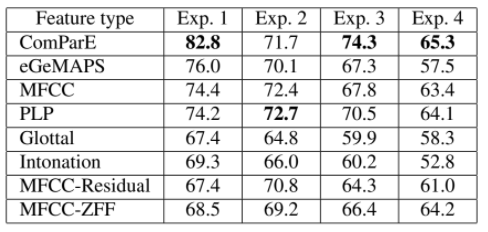
\includegraphics[width=\textwidth]{Feature wrt exp2.PNG}
    \\\tiny Source: \textit{Towards automatic assessment of voice disorders: A clinical approach (INTERSPEECH 2020)}
\end{frame}
\begin{frame}{Performance of voice disorder detection and assessment system}
\centering
    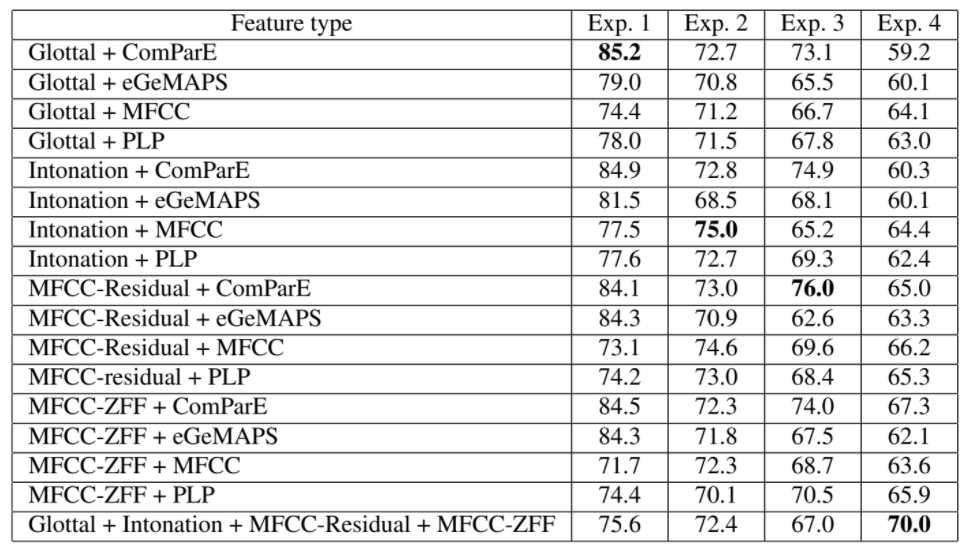
\includegraphics[width=\textwidth]{Feature wrt exp.PNG}
    \\\tiny Source: \textit{Towards automatic assessment of voice disorders: A clinical approach (INTERSPEECH 2020)}
\end{frame}
\begin{frame}{Inferences}
\begin{itemize}
    \item The classification of functional and \textbf{psychogenic} voice disorders is more challenging compared to classification of structural and neurogenic voice disorders. 
    \item Detection of voice disorder has a higher classification accuracy compared with the assessment of voice disorders
\end{itemize}
    
\end{frame}
\section{Methodology}
\begin{frame}{\small Machine Learning Life Cycle}
\centering
%\smartdiagrama[circular diagram]
   \smartdiagram[descriptive diagram]{
      {Define Objectives,{Voice Pathology, Sample Size,
              and Audio Features}},
      {Data, {Preprocesing,
                  labelling, sorting or frame conversion}},
      {Training, Feauture Extraction, Model Validation,
                 },
      {Evaluation, Accuracy,Feedback prediction, Performance comparison}}
\end{frame}
\begin{frame}{ML Concept}
\centering
      \smartdiagram[circular diagram]{Dataset Prep,
      Model Classifier, Transfer Learning, Verification, Monitor}
\end{frame}
\begin{frame}{Database}
    \begin{itemize}
        \item Saarbruecken Voice Disorder dataset which is \textcolor{red}{freely} available on \url{http://www.stimmdatenbank.coli.uni-saarland.de/}
        \item \textcolor{red}{2000} voice recordings sampled at 50 kHz: [Healthy ~ 428F+259M, Subject ~ 727F+629M]
        \item 71 different voice disorders
    \end{itemize}
\end{frame}
\begin{frame}{}
\centering
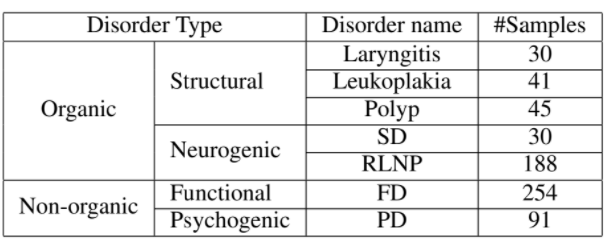
\includegraphics[width=9cm, height=6cm]{SVDsummary.PNG}
\end{frame}
\begin{frame}{}
\textbf{Feature: }Mel frequency cepstral coefficients of LP-residual, and ZFF signal
\begin{itemize}
    \item 39 dimensional cepstral coefficients consisting in 13 static coefficients, and their first and second order derivatives
    \item Modelling about 120+ dimensional vector. (156)
\end{itemize}
\textbf{Classifier:} Support vector machine (SVM) classifier is the most widely used classifier in voice disorder detection as it gives consistence performance even on small dataset. 
\end{frame}
\begin{frame}{Project Model: CNN-SVM}
\begin{enumerate}
    \item To develop a hybrid model of a powerful Convolutional Neural Networks (CNN) and Support Vector Machine (SVM) for detection.
    \item CNN works as an automatic feature extractor and SVM works as a binary classifier. 
\end{enumerate}
\begin{center}
    \textcolor{red}{SVM replaces the softmax layer of CNN}
\end{center}
%\tiny\textbf{Inspiration:}\textit{“Exploring Strategies for Training Deep Neural Networks.” Journal of Machine Learning Research}
\end{frame}
\begin{frame}{CNN Model}
\centering
    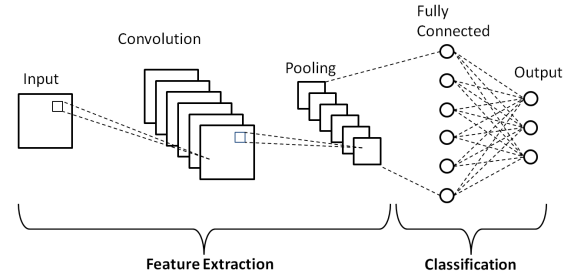
\includegraphics[width=9cm, height=6cm]{Simpleblock.PNG}
\end{frame}
\section{Works \& Planning Ahead}
\begin{frame}{Works Done so far}
\begin{itemize}
    \item \textbf{Literature Survey:}
    \begin{enumerate}
        \item Project Area's SWOT Analysis
        \item Scope for improvement [Literature or Algorithm]
    \end{enumerate}
\end{itemize}
    
\end{frame}
\begin{frame}{Works Done so far}
\begin{itemize}
    \item \textbf{Gathering Resources:}
    \begin{enumerate}
        \item Revise: Statistics, Calculus, Linear Algebra \& Probability
        \item Programming: Preprocessing data, feature extraction
        \item Model: Exploring other databases \& Classifiers 
    \end{enumerate}
\end{itemize}
    
\end{frame}
\begin{frame}{Works Done so far}
\begin{itemize}
    \item \textbf{Preparing Project Execution Steps:}
    \begin{enumerate}
        \item Contacting resource persons.
        \item Delegating task on a Gantt Chart.
    \end{enumerate}
\end{itemize}

\end{frame}
\begin{frame}{Current Status on Work}
\centering
    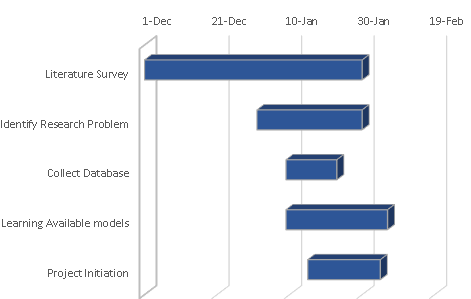
\includegraphics[width=\textwidth]{current status.PNG}
\end{frame}
\begin{frame}{Gantt Chart}
 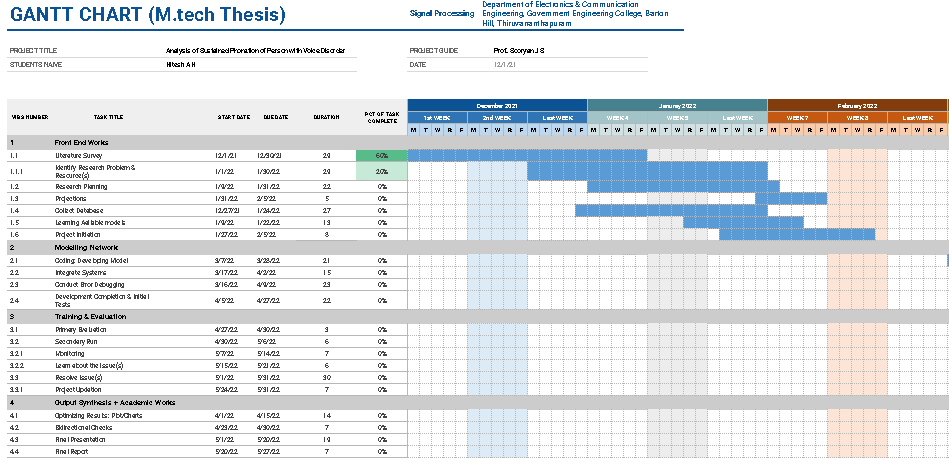
\includegraphics[width=\textwidth]{GanttChart1.PNG}
 \begin{center}
    \href{https://docs.google.com/spreadsheets/d/1GNJwdopzm6mXOZzkvvYEVpGXmIcgQHtT54OUhcYVjaM/edit?usp=sharing}{Click to View full Chart}
 \end{center}
\end{frame}
\begin{frame}
\frametitle{Retrospective}
\begin{itemize}
    \item Existing approaches are reactive post fixes to an outdated method.(\textcolor{red}{Monolithic Models})
    \item Modular Components have \colorbox{yellow}{clear} specification interface for individual feature.
    \item Building a reusable structure of learning is not a solution.
    \item Manual efforts are required in certain task(s). (Models \textcolor{red}{don't} communicate in between)
\end{itemize}
\end{frame}
\begin{frame}
\centering

\begin{tikzpicture}[scale=.132]

\pgfmathsetmacro {\goldenRatio} {(1+sqrt(5))}
\pgfmathsetmacro {\meanArea}
      {pow(\outerradius * 10 / \nbrcircles, 2) * pi}
\pgfmathsetmacro {\minArea} {\meanArea * (1 - \deviation)}
\pgfmathsetmacro {\midArea} {\meanArea * (1 + \deviation) - \minArea}

\foreach \b in {0,...,\nbrcircles}{
    % mod() must be used in order to calculate the right angle.
    % otherwise, when \b is greater than 28 the angle is greater
    % than 16384 and an error is raised ('Dimension too large').
    % -- thx Tonio for this one.
    \pgfmathsetmacro{\angle}{mod(\goldenRatio * \b, 2) * 180}

    \pgfmathsetmacro{\sratio}{\b / \nbrcircles}
    \pgfmathsetmacro{\smArea}{\minArea + \sratio * \midArea}
    \pgfmathsetmacro{\smRadius}{sqrt(\smArea / pi) / 2 * \fudge}
    \addtocounter{cumulArea}{\smArea};

    \pgfmathparse{sqrt(\value{cumulArea} / pi) / 2}
    \fill[] (\angle:\pgfmathresult) circle [radius=\smRadius] ;
}  
\end{tikzpicture}
\Huge{\centerline{Thank You}}
\end{frame}
%----------------------------------------------------------------------------------------
\end{document} 